\documentclass{article}
\usepackage[utf8x]{inputenc}
\usepackage[english]{babel}
\usepackage[T1]{fontenc}

%\usepackage[a4paper,top=3cm,bottom=2cm,left=2cm,right=2cm,marginparwidth=1.75cm]{geometry}
\usepackage[top=3.5cm, bottom=3.5cm, left=3.5cm, right=3.5cm]{geometry}
\usepackage{bm}
\usepackage{float}
\usepackage{amsmath}
\usepackage{graphicx}
\usepackage{fancyhdr}
\usepackage{listings}

\pagestyle{fancy}
\fancyhead[L]{SF2822: Applied Nonlinear Optimization}
\renewcommand{\headrulewidth}{1pt}
\fancyfoot[L]{}
\fancyfoot[C]{\thepage}
\fancyfoot[R]{}
\setlength{\headsep}{45pt}
\usepackage{enumitem}

\usepackage{tikz}
\usetikzlibrary{positioning}

\usepackage{amsfonts}

\begin{document}

\begin{titlepage}
\newcommand{\HRule}{\rule{\linewidth}{0.5mm}} 
\center 
\textsc{\LARGE KTH Royal Institute of Technology}\\[0.7cm]

\textsc{\Large SF2812 Applied Linear Optimization}\\[1cm]

\HRule \\[0.7cm]
{ \huge \bfseries Project 2B6 - Nonlinear Optimization Solver }\\[0.7cm]                            
\HRule \\[1cm]

\includegraphics[width=0.5\textwidth]{KTH_Logo.eps}\\[1cm]
\Large
\emph{Authors:}\\
Giovanni (940524-8551, cirillo@kth.se) \\
Martin (890313-0717, svedi@kth.se) \\
Yue Jiao (911024-7799, @kth.se)\\
\emph{Instructor:}\\
Anders Forsgren\\[0.5cm]
{\large May 2018}
\vfill 
\end{titlepage}

\lstset{language=Matlab,%
    %basicstyle=\color{red},
    breaklines=true,%
    morekeywords={matlab2tikz},
    keywordstyle=\color{blue},%
    morekeywords=[2]{1}, keywordstyle=[2]{\color{black}},
    identifierstyle=\color{black},%
    stringstyle=\color{mylilas},
    commentstyle=\color{mygreen},%
    showstringspaces=false,%without this there will be a symbol in the places where there is a space
    numbers=left,%
    numberstyle={\tiny \color{black}},% size of the numbers
    numbersep=9pt, % this defines how far the numbers are from the text
    emph=[1]{for,end,break},emphstyle=[1]\color{red}, %some words to emphasise
    %emph=[2]{word1,word2}, emphstyle=[2]{style},    
}



\newpage

\section{Basic problem}
\subsection{Problem description}
The goal is to construct a solver for the following type of problems:
\begin{equation} 
\begin{aligned}
\textrm{min} \quad        & \frac{1}{2} x^T H x + c^T x \\
\textrm{subject to} \quad & A x \geq b,  \\
                          & x \in \mathbb{R}^{n \times 1}
%                          & H \in \mathbb{R}^{n \times n} \\
%                          & c \in \mathbb{R}^{n \times 1} \\
%                          & A \in \mathbb{R}^{m \times n} \\
%                          & b \in \mathbb{R}^{m \times 1} \\
\end{aligned}
\label{prob:qp}
\end{equation}
where $H$ is assumed to be symmetric (if it is not, we can always make it symmetric and have an equivalent problem) and positive definite (if it is, our objective function is convex and the First order Necessary optimality conditions are also sufficient not only for local but also for global optimality).

\subsection{Solver algorithm}
We choose to solve this problem by an interior method solver. The full source code for our solver is available in the appendix.

We start by introducing slack variables $s$ for each inequality constraint in problem \ref{prob:qp}, giving us the following problem:
\begin{equation*} 
\begin{aligned}
\textrm{min} \quad        & \frac{1}{2} x^T H x + c^T x \\
\textrm{subject to} \quad & A x  - s = b,  \\
                          & s \geq 0 \\
                          & x \in \mathbb{R}^{n \times 1} \\
                          & s \in \mathbb{R}^{m \times 1}
%                          & H \in \mathbb{R}^{n \times n} \\
%                          & c \in \mathbb{R}^{n \times 1} \\
%                          & A \in \mathbb{R}^{m \times n} \\
%                          & b \in \mathbb{R}^{m \times 1} \\
\end{aligned}
\end{equation*}
The first order necessary optimality conditions for this problem then become:
\begin{equation*}
\begin{cases}
Hx-A^T\lambda=c\\
Ax-s=b\\
s_i \lambda_i=0 \quad i=1,2,...,m \\
s \ge 0 \\
\lambda \ge 0 \\
\end{cases}
\end{equation*}
%
This problem is hard to solve because of the complementarity condition $s_i \lambda_i=0 \quad i=1,2,...,m $. So we solve it approximately perturbing the optimality conditions putting a barrier parameter $\mu$.
%
\begin{equation*}
\begin{cases}
Hx-A^T\lambda=c\\
Ax-s=b\\
s_i \lambda_i=\mu \quad i=1,2,...,m \\
\end{cases}
\end{equation*}
In this case, the condition $s \geq 0$ and $\lambda \geq 0$ are kept implicitly by adapting the stepsize in the algorithm below.

Given $x$, $\lambda$ and $s$, we compute the corrections $\Delta x$, $\Delta \lambda$ and $\Delta s$:
%
\begin{equation}
\begin{cases}
H(x+\Delta x)-A^T(\lambda+\Delta \lambda)-c=0\\
A(x+\Delta x)-(s+\Delta s)-b=0\\
(s_i+\Delta s_i) (\lambda_i+\Delta \lambda_i)-\mu=0 \quad i=1,2,...,m \\
\end{cases}
\end{equation}
%
We linearize the last equation neglecting the term $\Delta s_i \Delta \lambda_i$ and we obtain the following system:
%
\begin{equation*}
\begin{bmatrix}
H & 0 & -A^T \\
A & -I & 0 \\
0 & \Lambda & S \\
\end{bmatrix} 
\begin{bmatrix}
\Delta x \\
\Delta s \\
\Delta \lambda \\
\end{bmatrix} 
 = - 
\begin{bmatrix}
H x + c - A^T \lambda \\
A x - s - b \\
S \Lambda e - \mu e
\end{bmatrix} 
\end{equation*}
%
where $S = diag(s)$, $\Lambda = diag(\lambda)$ and $e = (1, 1, ..., 1)^T$. 
So we compute the corrections and we multiply them by a proper parameter $\alpha \leq 1$ to satisfy also the implicit conditions .


In pseudocode the implemented solver performs the following steps:
%
\begin{enumerate}
\item Select a value of the barrier parameter $\mu > 0$. We choose $\mu = 1$. 

\item Given a initial value of the Lagrange multipliers vector $ \lambda \in \mathbb{R}^{m \times 1}, \quad \lambda > 0$ and of $x$ (the initial slack variables vector  $ s \in \mathbb{R}^{m \times 1}$ is calculated using $s_i=\mu/\lambda_i \quad i=1,2,...,m$; so, since both $\mu$ and $\lambda$ are greater than zero, also $s$ is greater than zero).

\item Compute the directions $\Delta x$, $\Delta s$ and $\Delta \lambda$ from the following equation.
%
\begin{equation*}
\begin{bmatrix}
H & 0 & -A^T \\
A & -I & 0 \\
0 & \Lambda & S \\
\end{bmatrix} 
\begin{bmatrix}
\Delta x \\
\Delta s \\
\Delta \lambda \\
\end{bmatrix} 
 = - 
\begin{bmatrix}
H x + c - A^T \lambda \\
A x - s - b \\
S \Lambda e - \mu e
\end{bmatrix} 
\end{equation*}
%
Where $S = diag(s)$, $\Lambda = diag(\lambda)$ and $e = (1, 1, ..., 1)^T$. 

\item Compute the maximum steplength $\alpha_{max}$ from $s + \alpha \Delta s \geq 0$, $\lambda + \alpha \Delta \lambda \geq 0$. 

\item Let $\alpha$ be a suitable step, $\alpha = \min{(1, \eta \alpha_{max})}$, where $\eta < 1$.  We have to choose a value for $\eta$ smaller than $1$ because, even though in the optimality conditions of the original problem we have $s\ge 0$ and $\lambda\ \ge 0$, in our case we must avoid the equality, otherwise we cannot solve our perturbed conditions. We choose $\eta = 0.99$.

\item Let $x = x + \alpha \Delta x$, $s = s + \alpha \Delta s$, $\lambda = \lambda + \alpha \Delta \lambda$.\\

\item We compute the new residual:

\begin{equation*}
\text{residual}=
\begin{bmatrix}
H x + c - A^T \lambda \\
A x - s - b \\
S \Lambda e -\mu e
\end{bmatrix} 
\end{equation*}

If the norm of the residual is smaller than a certain tolerance, for example $||\text{residual}||\le (n+2m) \mu$, we can reduce $\mu$ by a factor $10$, otherwise we keep the same $\mu$. Then return to step $3$.


\end{enumerate}

We repeat these steps until we reach convergence, for example when we reach $\mu<10^{-9}$.

\subsection{Sample problems}

We have tried to solve two different quadratic problems with linear inequality constraints.

\newpage

\textbf{Problem 1}

\begin{equation*} 
\begin{aligned}
\textrm{min} \quad        & x_1^2+x_1 x_2+2x_2^2-3x_1-36x_2 \\
\textrm{subject to} \quad & -x_1-x_2\geq -7,  \\
                          & x_1-5x_2\ge -25\\
                          & x_1 \ge 0\\
                          & x_2 \ge 0\\
\end{aligned}
\end{equation*}

From the problem we can get the various matrices and vectors that we need to put in our solver:

\begin{equation*}
H=
 \begin{bmatrix}
2 & 1 \\
1 & 4\\
\end{bmatrix} \succ 0
\quad c=
 \begin{bmatrix}
-3 \\
-36\\
\end{bmatrix} 
\quad A=
 \begin{bmatrix}
-1 & -1 \\
 1 & -5\\
 1 & 0\\
 0 & 1\\
\end{bmatrix} 
\quad b=
 \begin{bmatrix}
-7 \\
-25\\
 0\\
 0 \\
\end{bmatrix}
\end{equation*}

The advantage to use an interior point method is that we can choose the initial point arbitrarily, not necessarily feasible. But we have to choose $\lambda$ and $s$ greater than zero. So for example:

\begin{equation*}
x=
 \begin{bmatrix}
-1\\
1\\
\end{bmatrix} 
\quad \lambda=
 \begin{bmatrix}
 1 \\
 1\\
 1\\
 1\\
\end{bmatrix} 
\quad s=
 \begin{bmatrix}
 1 \\
 1\\
 1\\
 1\\
\end{bmatrix} 
\quad \mu=1
\end{equation*}



\textbf{Problem 2}

\begin{equation*} 
\begin{aligned}
\textrm{min} \quad        & x_1^2+x_1 x_2+\frac{3}{2}x_2^2+2x_3^2-4x_1-7x_2+4x_3 \\
\textrm{subject to} \quad & -x_1-x_2-x_3\geq -2,  \\
                          & -x_1+x_3\ge -1\\
                          & x_1 \ge 0\\
                          & x_3 \ge 0\\
\end{aligned}
\end{equation*}

From the problem we can get the various matrices and vectors that we need to put in our solver:
\begin{equation*}
H=
 \begin{bmatrix}
2 & 1 & 0 \\
1 & 3 & 0\\
0 & 0 & 4\\
\end{bmatrix} \succ 0
\quad c=
 \begin{bmatrix}
-4 \\
-7\\
4\\
\end{bmatrix} 
\quad A=
 \begin{bmatrix}
-1 & -1 & -1\\
 -1 & 0 & 1\\
 1 & 0 & 0\\
 0 & 0 & 1\\
\end{bmatrix} 
\quad b=
 \begin{bmatrix}
-2 \\
-1\\
 0\\
 0 \\
\end{bmatrix}
\end{equation*}


\begin{equation*}
x=
 \begin{bmatrix}
0\\
0\\
0\\
\end{bmatrix} 
\quad \lambda=
 \begin{bmatrix}
 1 \\
 1\\
 1\\
 1\\
\end{bmatrix} 
\quad s=
 \begin{bmatrix}
 1 \\
 1\\
 1\\
 1\\
\end{bmatrix} 
\quad \mu=1
\end{equation*}

\newpage

\subsection{Results and analysis}

\textbf{Problem 1}
\[
\begin{array}{ccccccccc} 
it & \mu & x_1 & x_2 & \lambda_1 & \lambda_2 & \lambda_3 & \lambda_4 & \text{residual}\\
\hline
0 & -- & -1.0 & 1.0 & 1.0 & 1.0 & 1.0 & 1.0 & 34.25\\ 1 & 1.0 & -0.6449 & 1.99 & 0.9116 & 1.295 & 1.123 & 0.01 & 26.35\\ 2 & 1.0 & 0.4979 & 4.761 & 0.8421 & 2.684 & 1.383 & 0.4279 & 6.8\\ 3 & 0.1 & 0.5939 & 5.1 & 0.03342 & 2.977 & 0.3598 & 0.004279 & 0.5831\\ 4 & 0.01 & 0.4976 & 5.099 & 0.004743 & 3.021 & 0.07817 & 0.001962 & 0.1083\\ 5 & 0.01 & 0.4753 & 5.094 & 0.007035 & 3.028 & 0.0236 & 0.001963 & 0.06257\\ 6 & 0.001 & 0.4694 & 5.094 & 0.0006675 & 3.031 & 0.002395 & 0.0001965 & 0.006153\\ 7 & 0.0001 & 0.4688 & 5.094 & 6.928\,{10}^{-5} & 3.031 & 0.0002162 & 1.963\,{10}^{-5} & 0.0006018\\ 8 & 1.0\,{10}^{-5} & 0.4688 & 5.094 & 6.954\,{10}^{-6} & 3.031 & 2.135\,{10}^{-5} & 1.963\,{10}^{-6} & 6.001\,{10}^{-5}\\ 9 & 1.0\,{10}^{-6} & 0.4688 & 5.094 & 6.956\,{10}^{-7} & 3.031 & 2.134\,{10}^{-6} & 1.963\,{10}^{-7} & 6.0\,{10}^{-6}\\ 10 & 1.0\,{10}^{-7} & 0.4688 & 5.094 & 6.956\,{10}^{-8} & 3.031 & 2.133\,{10}^{-7} & 1.963\,{10}^{-8} & 6.0\,{10}^{-7}\\ 11 & 1.0\,{10}^{-8} & 0.4688 & 5.094 & 6.957\,{10}^{-9} & 3.031 & 2.133\,{10}^{-8} & 1.963\,{10}^{-9} & 6.0\,{10}^{-8}\\ 12 & 1.0\,{10}^{-9} & 0.4688 & 5.094 & 6.957\,{10}^{-10} & 3.031 & 2.133\,{10}^{-9} & 1.963\,{10}^{-10} & 6.0\,{10}^{-9} \end{array}
\]

\medskip 
\textbf{Problem 2}
\[
\begin{array}{cccccccccc} 
it & \mu & x_1 & x_2 & x_3 & \lambda_1 & \lambda_2 & \lambda_3 & \lambda_4 & \text{residual}\\
\hline
0 & -- & 0 & 0 & 0 & 1.0 & 1.0 & 1.0 & 1.0 & 7.55\\ 1 & 1.0 & 0.2341 & 1.204 & -0.2743 & 1.448 & 1.508 & 1.482 & 1.99 & 3.416\\ 2 & 0.1 & 0.4419 & 1.525 & -0.007428 & 1.772 & 0.1841 & 0.4707 & 5.452 & 0.8198\\ 3 & 0.01 & 0.3764 & 1.616 & -0.0001663 & 1.764 & 0.001841 & 0.1404 & 5.757 & 0.1267\\ 4 & 0.01 & 0.3369 & 1.656 & 0.001756 & 1.697 & 0.01592 & 0.04176 & 5.688 & 0.06924\\ 5 & 0.001 & 0.3334 & 1.666 & 0.0001817 & 1.669 & 0.001459 & 0.003397 & 5.669 & 0.006554\\ 6 & 0.0001 & 0.3333 & 1.667 & 1.77\,{10}^{-5} & 1.667 & 0.0001502 & 0.0003007 & 5.667 & 0.0006044\\ 7 & 1.0\,{10}^{-5} & 0.3333 & 1.667 & 1.765\,{10}^{-6} & 1.667 & 1.5\,{10}^{-5} & 3.0\,{10}^{-5} & 5.667 & 6.003\,{10}^{-5}\\ 8 & 1.0\,{10}^{-6} & 0.3333 & 1.667 & 1.765\,{10}^{-7} & 1.667 & 1.5\,{10}^{-6} & 3.0\,{10}^{-6} & 5.667 & 6.0\,{10}^{-6}\\ 9 & 1.0\,{10}^{-7} & 0.3333 & 1.667 & 1.765\,{10}^{-8} & 1.667 & 1.5\,{10}^{-7} & 3.0\,{10}^{-7} & 5.667 & 6.0\,{10}^{-7}\\ 10 & 1.0\,{10}^{-8} & 0.3333 & 1.667 & 1.765\,{10}^{-9} & 1.667 & 1.5\,{10}^{-8} & 3.0\,{10}^{-8} & 5.667 & 6.0\,{10}^{-8}\\ 11 & 1.0\,{10}^{-9} & 0.3333 & 1.667 & 1.765\,{10}^{-10} & 1.667 & 1.5\,{10}^{-9} & 3.0\,{10}^{-9} & 5.667 & 6.0\,{10}^{-9} \end{array}
\]

We notice that the number of iteration is very low, so the method converges quite fast. After only $5$ or $6$ iterations we have a solution that is accurate up to the fourth decimal digit. The number of iterations doesn't change much even if we increase the dimension of our problem.

For problem one, since the $x$ is 2-dimensional, we can also plot the result.

\begin{figure}[H]
    \centering
    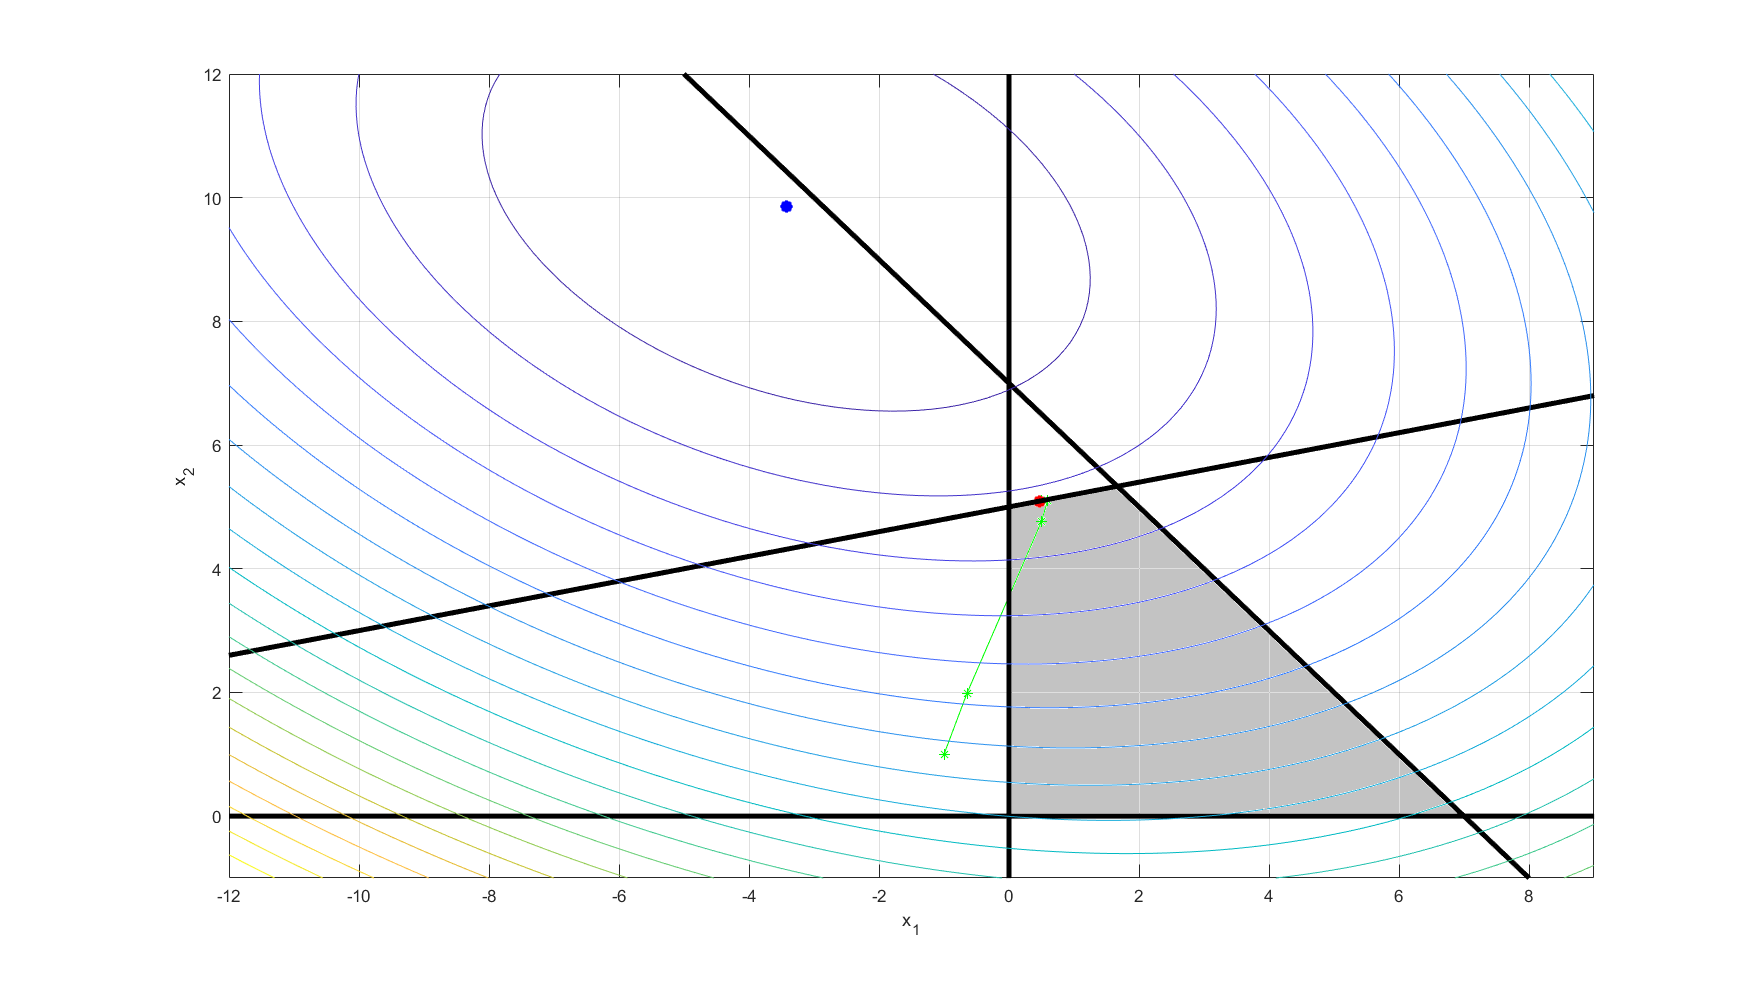
\includegraphics[width=16cm]{fig1_qp.png}
    \caption{Graphical solution problem 1: the feasible region is grey, the green line represent our path, the red point is our approximate solution when we reach convergence, while the blue point is the optimal solution of the unconstrained problem }.
\end{figure}



\newpage

\section{Advanced problem}
\subsection{Problem description}
In this part we aim at constructing a SQP solver for the following type of problems:
\begin{equation}
\begin{aligned}
\textrm{min} \quad        & f(x) \\
\textrm{subject to} \quad & g_i(x) \geq 0 \quad i = 1, .., m \\
                          & x \in \mathbb{R}^n
\end{aligned}
\label{prob:sqp}
\end{equation}
where $f$ and each $g_i$ is assumed to be at least twice continuously differentiable. Additionally, we require that the problem be such that  $\nabla^2_{xx}\mathcal{L}(x, \lambda)$ is positive definite.

\subsection{Solver algorithm}
Let the Lagrangian function of this problem be defined as:
\begin{equation*}
    \mathcal{L}(x, \lambda) = f(x) - \lambda^T g(x) 
\end{equation*}
Then the first-order optimality conditions are:

\begin{equation*}
    \begin{cases}
    \nabla_x \mathcal{L}(x, \lambda) = \nabla f(x) -A(x)^T \lambda = 0 \qquad \lambda \ge 0\\
    -\nabla_\lambda \mathcal{L}(x, \lambda) = g(x) \ge 0
    \end{cases}
\end{equation*}
where $A(x)^T=[\nabla g_1(x), \nabla g_2(x),...,\nabla g_m(x)]$.

% To express the inequality in a linear equation, a slack variable $s$ is added. Thus we have the following linear equation. 
% If we add the slack variables $s$, we have this optimality conditions:


% \begin{equation*}
%     \begin{cases}
%     \nabla f(x) -A(x)^T \lambda = 0 \qquad \lambda \ge 0\\
%     g(x)-s = 0 \qquad s \ge 0\\
%     \lambda_i s_i=0 \quad i=1,2,...,m
%     \end{cases}
% \end{equation*}

A Newton iteration for solving the first-order necessary
optimality conditions may be viewed as solving the QP
problem:
\begin{equation*}
\begin{aligned}
\textrm{minimize } \frac{1}{2} p^T\nabla^2_{xx}\mathcal{L}(x, \lambda)p + \nabla f(x)^T p \\
\textrm{subject to } A(x) p \geq -g(x)
\end{aligned}
\end{equation*}
But now we can solve this problem using our QP-solver by setting $H=\nabla^2_{xx}\mathcal{L}(x, \lambda)$, $c=\nabla f(x)$, $A=A(x)$, $b=- g(x)$.

Solving this problem we find the optimal solution of $p$ and $\lambda$ for our quadratic problem. This $\lambda$ is relative to the QP, so we call it $\lambda_{QP}$. Then we can use $p$ and $\lambda_{QP}$ to update the values of $x$ and $\lambda_{NLP}$ relative to our original non-linear problem. In the following pages, when we say $\lambda$ without any subscript,we refer to $\lambda_{NLP}$. Actually our solver gives us also the slack variables $s$, which is related to the quadratic subproblem, so we call it $s_{QP}$, that we use to update the $s_{NLP}$ of the original non-linear problem, that we call simply $s$.

Thus the sequential quadratic programming algorithm is described as below.
\begin{enumerate}
    \item Choose a starting point of $x$ and $\lambda$ for the non linear problem. 
    \item Evaluate $\nabla^2_{xx}\mathcal{L}(x, \lambda)$, $\nabla f(x)$, $A(x)$ and $-g(x)$ in our point ($x$, $\lambda$).
    \item Choose a starting point of $p$ and $\lambda_{QP}$ for the quadratic problem. 
    \item Calculate the steps $p$ and $\lambda_{QP}$ with the equation 2 above. 
    \item Update $x \rightarrow x + p$, $\lambda \rightarrow \lambda_{QP}$ and $s \rightarrow s_{QP}$
    \item We compute the residual:
    \begin{equation*}
\text{residual}=
\begin{bmatrix}
\nabla f(x)-A(x)^T \lambda  \\
g(x)-s \\
\lambda^T g(x)\\
\end{bmatrix} 
\end{equation*}

If the norm of this residual is less than a certain value, for example $10^{-7}$, we can stop the iterations, otherwise we can go back to step 2.
An important thing to remember is to choose the tolerances for the residual wisely. In fact, if we solve each subproblem with a tolerance of the order of $10^{-9}$ we cannot obtain a tolerance for the original non linear problem that is better, so if we choose too similar tolerances we could enter in an infinite loop. To avoid that, we decide to have a tolerance for the non linear problem which is two order of magnitude higher than for the corresponding subproblems.


\end{enumerate}


\subsection{Sample problems}
\subsubsection{Problem 1}
The problem is to:
\begin{equation*}
\begin{aligned}
\textrm{min } & 4(x_1-2)^2 + (x_2-1)^2 \\
\textrm{subject to } & 1 - x_1^2 - x_2^2 \geq 0 \\
                     & 4 - x_1^2 - (x_2-2)^2 \geq 0 \\
\end{aligned}
\end{equation*}

Let the objective function be $f =  4(x_1-2)^2 + (x_2-1)^2 $. Then $\nabla f = \begin{bmatrix} 8x_1-16\\ 2x_2-2 \\ \end{bmatrix}$. Let $g_1(x) = 1 - x_1^2 - x_2^2 $ and $g_2 = 4 - x_1^2 - (x_2-2)^2$. Then $\nabla g_1(x) = \begin{bmatrix} -2x_1\\ -2x_2 \\ \end{bmatrix}$ and $\nabla g_2(x) = \begin{bmatrix} -2x_1 \\ -2x_2+4 \\ \end{bmatrix}$. The Hessian of the Lagrangian function is given by the following: 
\begin{equation*}
    H(\mathcal{L}(x, \lambda)) = H(f(x)) - \sum_{i=1}^2 \lambda_i^T H(g_i) = \begin{bmatrix} 8 &  0\\ 0 & 2 \\ \end{bmatrix} - \lambda_1 \begin{bmatrix} -2 & 0\\ 0 & -2 \\ \end{bmatrix} - \lambda_2 \begin{bmatrix} -2 & 0\\ 0 & -2 \\ \end{bmatrix}
\end{equation*}
We can see that the problem is convex , since the objective function is convex (the Hessian of the objective function is positive definite) and the inequality constraints are concave (the Hessians of the constraints are negative definite). So our QP-solver can be used to find a global optimal solution.

The initial value of $x$ and $\lambda$ are $x = [-5, -3]^T$ and $\lambda = [1, 1]^T$. 


\subsubsection{Problem 2}
The problem is to:
\begin{equation*}
\begin{aligned}
\textrm{min } & \frac{1}{2}(x_1+1)^2+\frac{1}{2}(x_2+2)^2 \\
\textrm{subject to } & 6 - 3(x_1+x_2-2)^2 - (x_1-x_2)^2 \ge 0 \\
                     & x_1 \geq 0 \\
                     & x_2 \geq 0 \\ 
\end{aligned}
\end{equation*}

Let the objective function be $f =  \frac{1}{2}(x_1+1)^2+\frac{1}{2}(x_2+2)^2 $. Then $\nabla f = \begin{bmatrix} x_1+1\\ x_2+2 \\ \end{bmatrix}$. Let $g_1(x) = 6-3(x_1+x_2-2)^2-(x_1-x_2)^2 $, $g_2 = x_1$ and $g_3 = x_2$. Then $\nabla g_1(x) = \begin{bmatrix} -4(2x_1+x_2-3) \\  -4(x_1+2x_2-3) \\ \end{bmatrix}$, $\nabla g_2(x) = \begin{bmatrix} 1 \\ 0 \\ \end{bmatrix}$ and $\nabla g_3(x) = \begin{bmatrix} 0 \\ 1 \\ \end{bmatrix}$. The Hessian of the Lagrangian function is given by the following: 
\begin{equation*}
    H(\mathcal{L}(x, \lambda)) = H(f(x)) - \sum_{i=1}^3 \lambda_i^T H(g_i) = \begin{bmatrix} 1 &  0\\ 0 & 1 \\ \end{bmatrix} - \lambda_1 \begin{bmatrix} -8 & -4\\ -4 & -8 \\ \end{bmatrix} - \lambda_2 \begin{bmatrix} 0 & 0\\ 0 & 0 \\ \end{bmatrix} - \lambda_3 \begin{bmatrix} 0 & 0\\ 0 & 0 \\ \end{bmatrix}
\end{equation*}

We can see that the problem is convex, since the objective function is convex (the Hessian of the objective function is positive definite) and the inequality constraints are concave (the Hessians of the first constraint is negative definite) or linear (the second and the third constraint). So our QP-solver can be used to find a global optimal solution.

The initial value of $x$ and $\lambda$ are $x = [2, -3]^T$ and $\lambda= [1, 1, 1]^T$. 


\subsubsection{Problem 3}
The problem is to:
\begin{equation*}
\begin{aligned}
\textrm{min } & e^{(x_1+x_2)}+x_1^2+x_1x_2+2x_2^2+x_1 \\
\textrm{subject to } & 10-x_1^2-x_2^2 \geq 0 \\
                     & x_2 \geq 1 \\
\end{aligned}
\end{equation*}

Let the objective function be $f =  e^{(x_1+x_2)}+x_1^2+x_1*x_2+2x_2^2+x_1$. Then $\nabla f = \begin{bmatrix} e^{(x_1+x_2)}+2x_1+x_2+1\\ e^{(x_1+x_2)}+x_1+4x_2 \\ \end{bmatrix}$. Let $g_1(x) = 10-x_1^2-x_2^2 $ and $g_2 = x_2-1$. Then $\nalba g_1(x) = \begin{bmatrix} -2x_1\\ -2x_2\\ \end{bmatrix}$ and $\nabla g_2(x) = \begin{bmatrix} 0 \\ 1 \\ \end{bmatrix}$. The Hessian of the Lagrangian function is given by the following: 
\begin{equation*}
    H(\mathcal{L}(x, \lambda)) = H(f(x)) - \sum_{i=1}^2 \lambda_i^T H(g_i) = \begin{bmatrix} e^{(x_1+x_2)}+2 &  e^{(x_1+x_2)}+1 \\ e^{(x_1+x_2)}+1 & e^{(x_1+x_2)}+4 \\ \end{bmatrix} - \lambda_1 \begin{bmatrix} -2 & 0\\ 0 & -2\\ \end{bmatrix}- \lambda_2 \begin{bmatrix} 0 & 0\\ 0 & 0 \\ \end{bmatrix}
\end{equation*}

We can see that the problem is convex, since the objective function is convex (the Hessian of the objective function is positive definite) and the inequality constraints are concave (the Hessian of the first constraint is negative definite) or linear (the second constraint). So our QP-solver can be used to find a global optimal solution.

Actually in our case the Hessian of the objective function is not constant (it depends on the point that we consider), but we can see that the matrix is strictly diagonally dominant, so it is positive definite.

The initial value of  $x$ and $\lambda$ are $x = [0, 0]^T$ and $\lambda = [1, 1]^T$. 



\subsubsection{Problem 4}
Now we see what happens if the problem is not convex
The problem is to:
\begin{equation*}
\begin{aligned}
\textrm{min } & (x_1-1)(x_1-2)(x_2-1)(x_2-2) \\
\textrm{subject to } & 1-x_1^2-x_2^2 \geq 0 \\
\end{aligned}
\end{equation*}

Let the objective function be $f = (x_1-1)(x_1-2)(x_2-1)(x_2-2)$. Then

$\nabla f = \begin{bmatrix} (2x_1-3)(x_2^2-3x_2+2) \\ (2x_2-3)(x_1^2-3x_1+2) \end{bmatrix}$. 

Let $g(x) = 10-x_1^2-x_2^2 $. Then $\nabla g(x) = \begin{bmatrix} -2x_1\\ -2x_2\\ \end{bmatrix}$  The Hessian of the Lagrangian function is given by the following: 
\begin{equation*}
    H(\mathcal{L}(x, \lambda)) = H(f(x)) -  \lambda_i^T H(g) = H(f(x)) - \lambda \begin{bmatrix} -2 & 0\\ 0 & -2\\ \end{bmatrix}
\end{equation*}

where:

$H_{11}(f(x))= 2(x_2-2)(x_2-1)$

$H_{12}(f(x))=H_{21}(f(x))=(x_1-2)(x_2-2)+(x_1-1)(x_2-2)+(x_1-2)(x_2-1)+(x_1-1)(x_2-1)$

  $H_{22}(f(x))=    2(x_1-2)(x_1-1)$ 

\medskip

The problem is not convex, because the Hessian of the objective function is not positive definite in all the points, but we can say that inside our feasible region the objective function is positive everywhere except in two points, where it is zero, at $x=(0,1)$ and $x=(1,0)$.
So both these points are local optima.
If we run our code, we notice that if the starting point is sufficiently close to the first local optimum we converge to that point, if the starting point is sufficiently close to the second local optimum we converge to that point, while if we are far from both these points, the Hessian of the Lagrangian is not positive definite, so our QP-solver doesn't work.

\subsection{Result and analysis}

Here we show only the iterations of the outer program, not the inner one. So remember that from one iteration and the following there are all the iterations of the inner program (the quadratic one).

\bigskip

\textbf{Problem 1}
\[
\begin{array}{cccccc} 
it &  x_1 & x_2  & \lambda_1 & \lambda_2 & \text{residual}\\
\hline
0 & -5.0 & -3.0 & 1.0 & 1.0 & 98.6\\ 1 & -0.3333 & -1.667 & 4.615\,{10}^{-11} & 7.143\,{10}^{-11} & 38.56\\ 2 & 2.0 & 1.0 & 1.169\,{10}^{-10} & 8.654\,{10}^{-11} & 17.76\\ 3 & 1.375 & 0.25 & 1.0 & 0.25 & 3.032\\ 4 & 1.028 & 0.25 & 3.124 & 0.01769 & 1.375\\ 5 & 0.97 & 0.25 & 4.037 & 0.1481 & 0.1228\\ 6 & 0.9682 & 0.25 & 4.104 & 0.1578 & 0.0002734\\ 7 & 0.9682 & 0.25 & 4.105 & 0.1578 & 2.049\,{10}^{-9} \end{array}
\]



\begin{figure}[H]
    \centering
    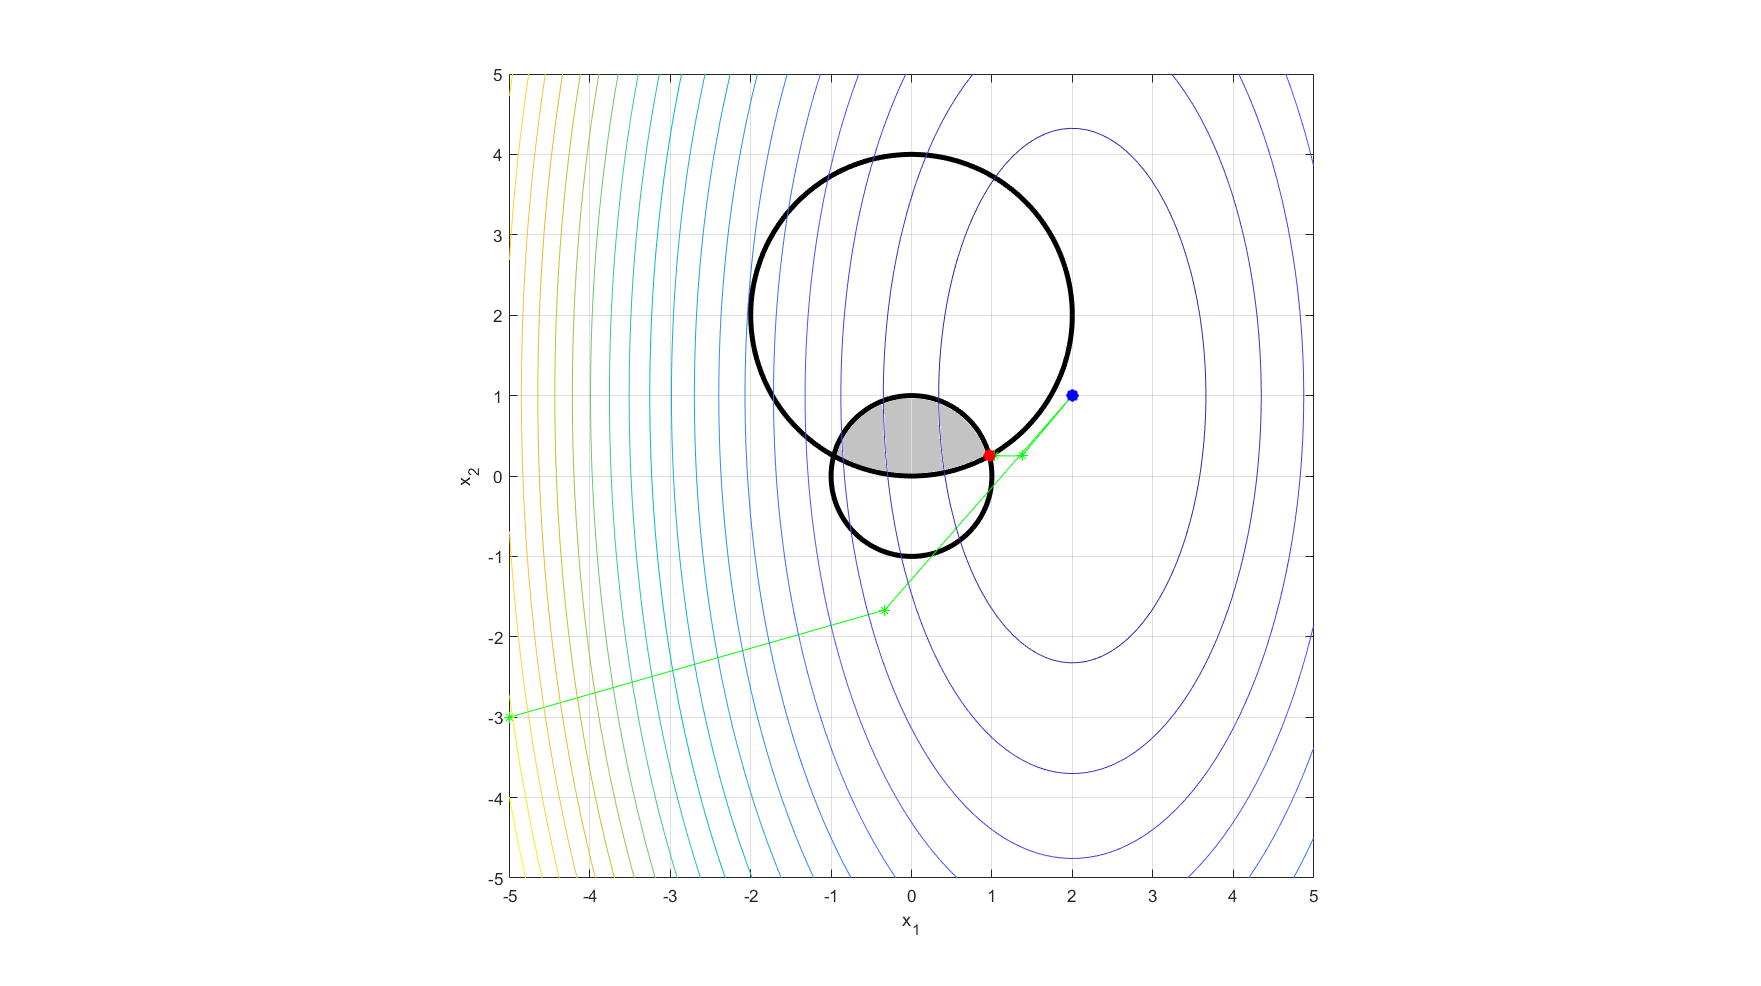
\includegraphics[width=16cm]{fig1_sqp.png}
    \caption{Graphical solution problem 1: the feasible region is grey, the green line represent our path, the red point is our approximate solution when we reach convergence, while the blue point is the optimal solution of the unconstrained problem }
\end{figure}

As the iterations go, the points move from outside of the feasible region to the inside and finally reach the optimal point. 

\bigskip


\textbf{Problem 2}
\[
\begin{array}{ccccccc} 
it &  x_1 & x_2  & \lambda_1 & \lambda_2 & \lambda_3 & \text{residual}\\
\hline
 0 & 2.0 & -3.0 & 1.0 & 1.0 & 1.0 & 56.31\\ 1 & 0.3333 & 5.172\,{10}^{-11} & 4.054\,{10}^{-11} & 3.0\,{10}^{-9} & 19.33 & 32.21\\ 2 & 0.5952 & 5.654\,{10}^{-9} & 0.1709 & 1.68\,{10}^{-9} & 0.1769 & 0.4854\\ 3 & 0.5732 & 0.04509 & 0.2175 & 1.745\,{10}^{-9} & 2.218\,{10}^{-8} & 0.01408\\ 4 & 0.5767 & 0.04308 & 0.2185 & 1.734\,{10}^{-9} & 2.321\,{10}^{-8} & 4.173\,{10}^{-5}\\ 5 & 0.5767 & 0.04309 & 0.2185 & 1.734\,{10}^{-9} & 2.321\,{10}^{-8} & 3.01\,{10}^{-9} \end{array}
\]

\begin{figure}[H]
    \centering
    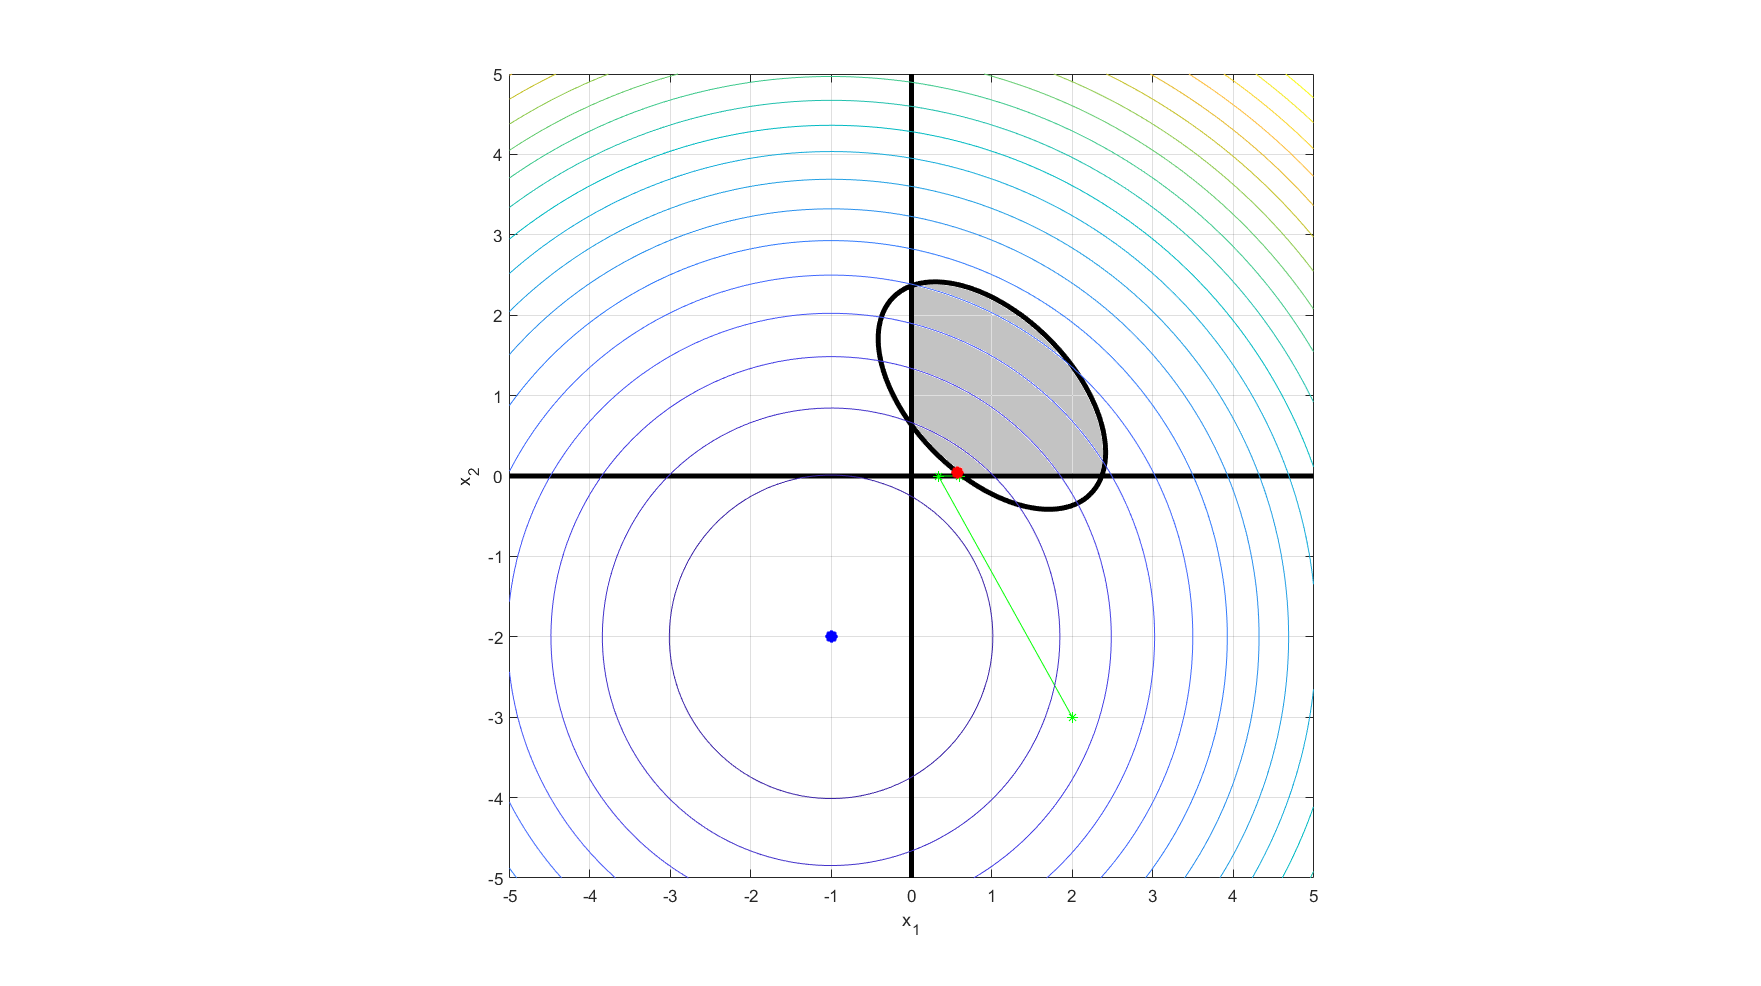
\includegraphics[width=16cm]{fig2_sqp.png}
    \caption{Graphical solution problem 2: the feasible region is grey, the green line represent our path, the red point is our approximate solution when we reach convergence, while the blue point is the optimal solution of the unconstrained problem }
\end{figure}
\bigskip


\textbf{Problem 3}\\
\[
\begin{array}{cccccc}
it &  x_1 & x_2 & \lambda_1 & \lambda_2  & \text{residual}\\
\hline
0 & -2.0 & 3.0 & 1.0 & 1.0 & 18.35\\ 1 & -1.473 & 1.316 & 1.086\,{10}^{-10} & 3.161\,{10}^{-9} & 5.598\\ 2 & -1.346 & 1.0 & 1.369\,{10}^{-10} & 3.346 & 0.1178\\ 3 & -1.352 & 1.0 & 1.394\,{10}^{-10} & 3.352 & 3.204\,{10}^{-5}\\ 4 & -1.352 & 1.0 & 1.394\,{10}^{-10} & 3.352 & 2.0\,{10}^{-9} \end{array}
\]







\begin{figure}[H]
    \centering
    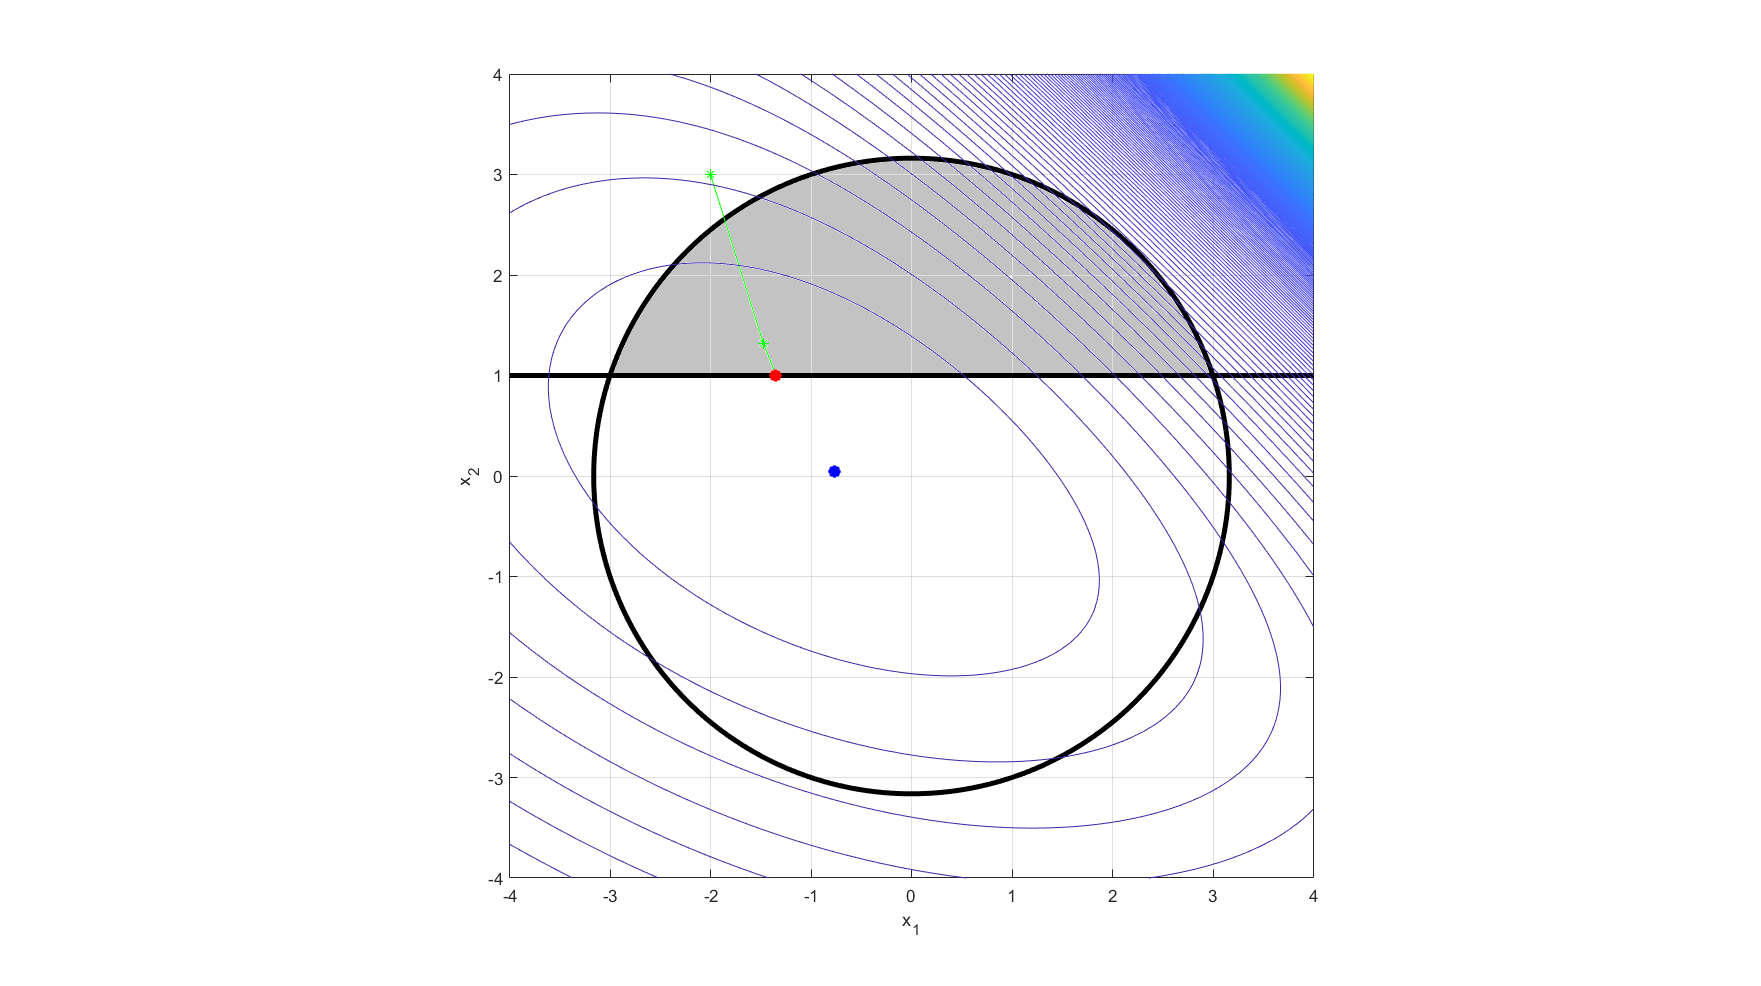
\includegraphics[width=16cm]{fig3_sqp.png}
    \caption{Graphical solution problem 3: the feasible region is grey, the green line represent our path, the red point is our approximate solution when we reach convergence, while the blue point is the optimal solution of the unconstrained problem }
\end{figure}

\textbf{Problem 4 (using different starting points)}
\[
\begin{array}{ccccc} 
it &  x_1 & x_2 & \lambda & \text{residual}\\
\hline
0 & 0.9 & 0.3 & 1.0 & 1.436\\ 1 & 1.079 & -0.06977 & 0.9499 & 0.2674\\ 2 & 1.005 & -0.007842 & 1.006 & 0.01923\\ 3 & 1.0 & -0.0001034 & 1.0 & 0.00024\\ 4 & 1.0 & -2.105\,{10}^{-8} & 1.0 & 3.793\,{10}^{-8}\\ 5 & 1.0 & 7.5\,{10}^{-10} & 1.0 & 1.0\,{10}^{-9} \end{array}
\]

Here we converge to the point $x=(1,0)$ and $\lambda=1$.

\bigskip

\[
\begin{array}{ccccc}
it &  x_1 & x_2 & \lambda & \text{residual}\\
\hline
0 & 0.3 & 0.9 & 1.0 & 1.436\\ 1 & -0.06977 & 1.079 & 0.9499 & 0.2674\\ 2 & -0.007842 & 1.005 & 1.006 & 0.01923\\ 3 & -0.0001034 & 1.0 & 1.0 & 0.00024\\ 4 & -2.105\,{10}^{-8} & 1.0 & 1.0 & 3.793\,{10}^{-8}\\ 5 & 7.5\,{10}^{-10} & 1.0 & 1.0 & 1.0\,{10}^{-9} \end{array}
\]

Here we converge to the point $x=(0,1)$ and $\lambda=1$.

\[
\begin{array}{ccccc}
it &  x_1 & x_2 & \lambda & \text{residual}\\
\hline
0 & 0.5 & 1.2 & 1.0 & 3.066\\ 1 & 0.04819 & 1.101 & 0.5581 & 0.4594\\ 2 & 0.04819 & 1.101 & 1.0 & 1.766 \end{array}
\]

Here we stop because the Hessian of the Lagrangian is not positive definite anymore, so the solution is not correct (we see that the residual is very large).

\newpage

\section*{Appendix: Matlab Code (qp\_algorithm.m)}

\lstinputlisting{qp_algorithm.m}

\end{document}